%! Author: Henrik Agerholm Ferrari, Þorvaldur Máni Danivalsson, Fei Gu
% This is the EASV CS21 4th Semester IOT Exam project report.
% Group name is


% Preamble
\documentclass[12pt, a4, utf8]{report}        % here is the document's type which is {article}.
\title{Making a new tomorrow in cyber stalking and e worms}                                   % the title of this document.
\author{Smarty pants: Henrik Agerholm Ferrari, Þorvaldur Máni Danivalsson, Fei Gu}
\date{\today}

% Packages
\usepackage{amsmath}
\usepackage{graphicx}
\usepackage{blindtext}


% Document
\begin{document}        % the ducument start here
    \maketitle
    \tableofcontents


    \section{Problem statement}\label{sec:problem-statement}
    % Which problem for a human is it solving and why is it important
    \blindtext{}


    \section{Illustration of network architecture}\label{sec:illustration-of-network-architecture}
    % Use draw.io make a architecture, remember to name the protocols and the hardwares.


    \paragraph{}
    Following the problem statement, we have to design the architecture base on three different terminal using three ESP32 MCU.


    \paragraph{}
    The first terminal which connect to the all sensor component will try to get the data.
    And then when the data value reach to a limit then send a message to MQTT server by Wi-Fi connection, at the
    same time send the data to "Blynk.console" to show the data.


    \paragrapg{}
    The MQTT server will subscribe the topic

    \blindtext{}

    \section{Illustration of the hardware setup}\label{sec:illustration-of-the-hardware-setup}
    % Use fritzing or just use circuiTikZ make the circuit layout\pm
    \paragraph{}
    This part will explain the circuit and wire connection.

    \blindtext{}


    \subsection{esp32No1 Sensor}\label{subsec:esp32no1-sensor}
    \paragraph{}
    This is the part ESP32 to connect to the sensors.

    \blindtext{}



    \begin{figure}[h]
        \caption{ESP32 no.1 connect to sensors}
        \centering
        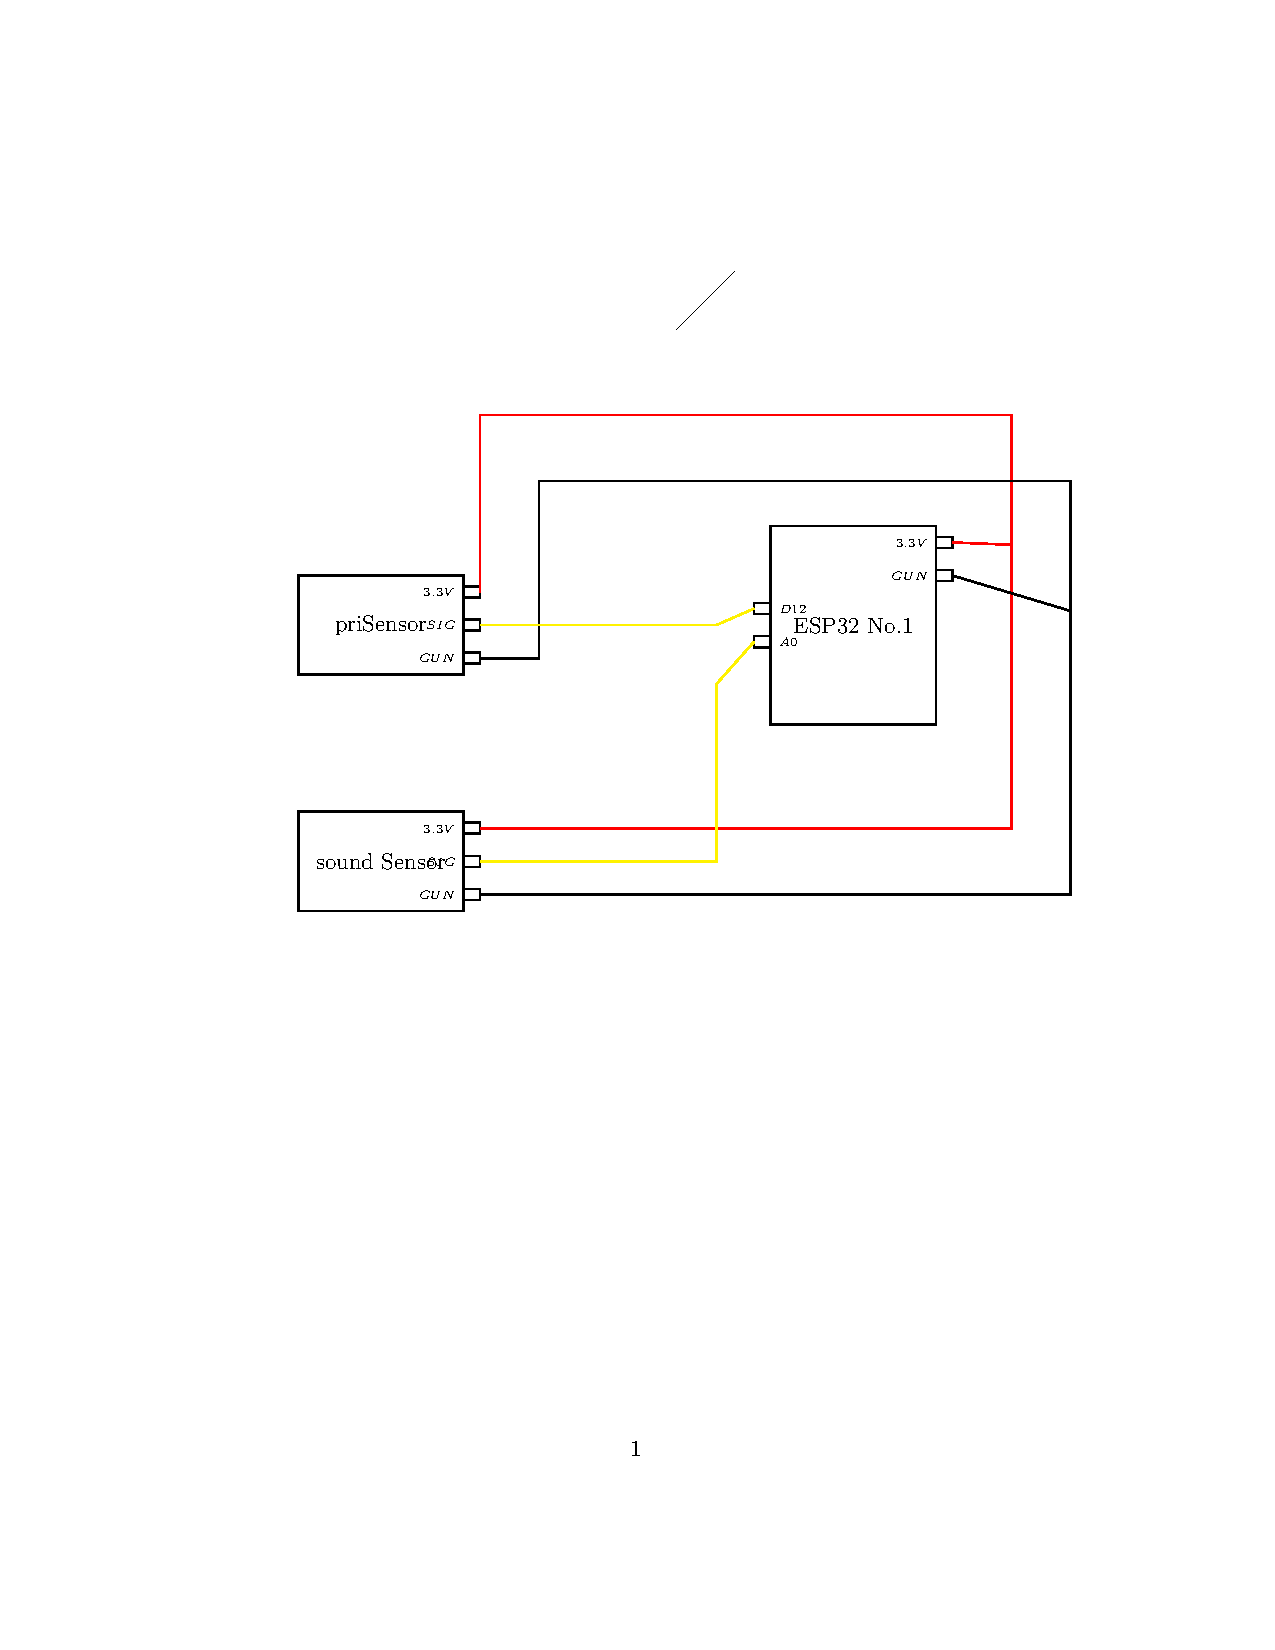
\includegraphics[width=0.5\textwidth]{../out/ESP32_No1_connect_Sensor}
        \label{fig:figure2}
    \end{figure}


    \subsection{esp32No2 Buzzer}\label{subsec:esp32no2-buzzer}
    \paragraph{}
    This part is talking about the ESP32 connect to the buzzer.
    this is a quite simple circuit we connect the 3.3 to power and gun to gun.
    and then connect the sig pin to D12 to set the data trans.

    \blindtext{}



    \begin{figure}[h]
        \caption{ESP32 no.2 connect to buzzer and LED-display}\label{fig:figure3}
        \centering
        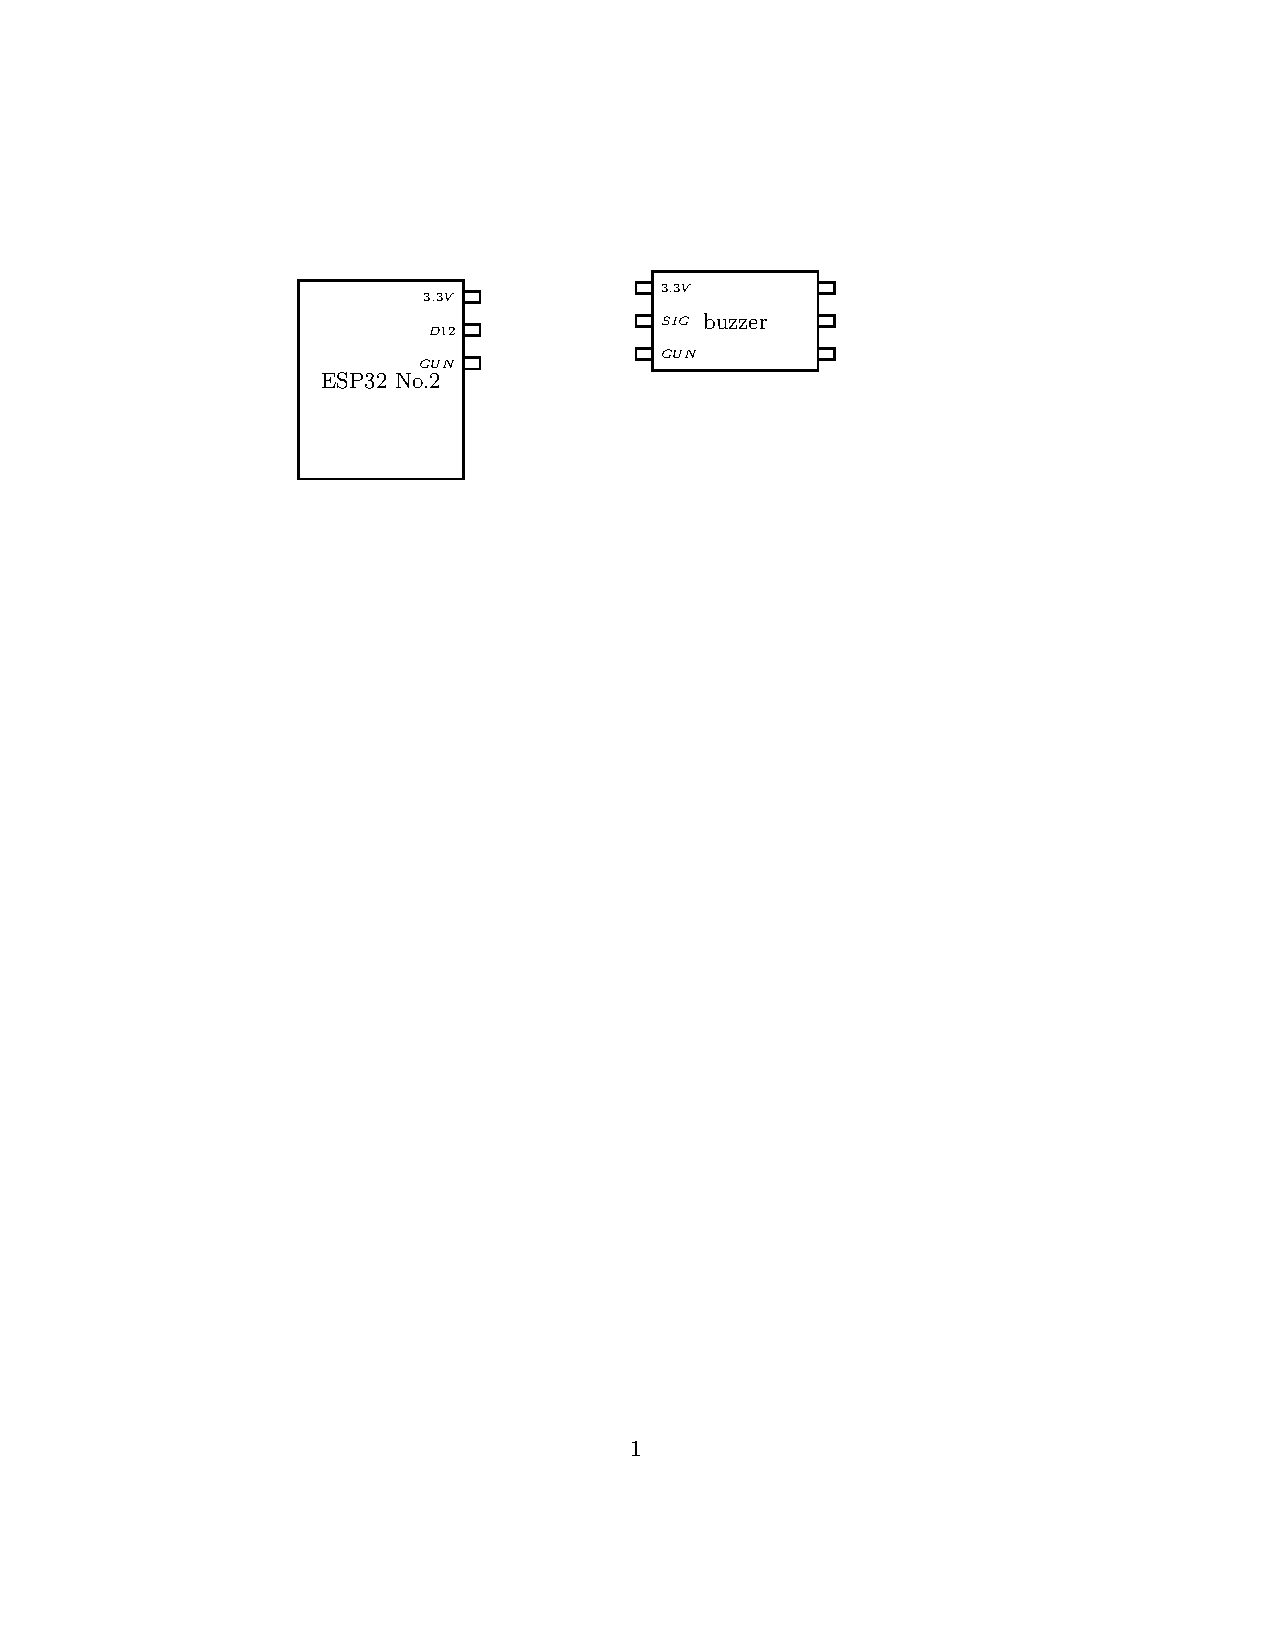
\includegraphics[width=0.5\textwidth]{../out/ESP32_No.2_connect_Buzzer}
    \end{figure}

    \subsection{esp32Cam }\label{subsec:esp32cam}
    \paragraph{}
    This part is the connection about the Esp32 Camera can be flash under the develop mode.
    And when we leave the development mode then just unplug all the wires except the power and ground.

    \blindtext{}



    \begin{figure}[h]
        \caption{ESP32 CAM}\label{fig:figure4}
        \centering
        \includegraphics[width=0.5\textwidth]{../out/ESP32Cam_connect_TypeCAdapter}
    \end{figure}



    \bibliography{report}
    \bibliographystyle{plain}

\end{document}
